% =======================================================================
\section{Introduction}
\label{sec:intro}

A team of learning agents can fail even when the task has a good cooperative solution: instead of
learning complementary behavior, agents can settle into locally safe, low-cooperation behaviour.
We call this \emph{coordination collapse};
in the MARL literature its endpoint is the \emph{lazy-agent}
policy~\citep{liu2023lazy,peng2023curo}, and the underlying private-versus-collective conflict is
the one studied in sequential social dilemmas~\citep{leibo2017multi}. We study this failure through
a \emph{reward-centralization} dial: within each reward-mixing sweep, agent $i$ is trained on the
blended scalar $x_i(w)=(1-w)\,r_i^{\mathrm{local}}+w\,r^{\mathrm{global}}$, $w\in[0,\allowbreak 1]$, so at
$w{=}0$ the learner sees only its own local reward and at $w{=}1$ only the team reward. Turn $w$
down and an agent's private performance drowns out its contribution; cooperating earns no
learnable signal and the lazy policy wins. That decentralized reward shaping cannot match
centralized training is broadly accepted~\citep{dmarl2025}, and lazy-agent and credit-assignment
work~\citep{liu2023lazy,peng2023curo,sunehag2018vdn,rashid2018qmix,foerster2018counterfactual}
mitigates the pathology; what none of it supplies is the \emph{location}. The closest phase-diagram
studies place their critical points on \emph{environmental}~\citep{yamaguchi2025} or
opinion-dynamics~\citep{capannoli2026phase} axes rather than reward structure, and none estimates a
confidence-intervalled crossing in reward-centralization space for gradient-trained cooperative
policies. Our central question is therefore twofold: does coordination collapse admit a
\emph{measurable} finite-budget behavioral crossing $\wcrit$, and how do reward transformations,
including their scale, move that crossing? The first is the paper's primary measurement problem;
the second is an application that also tests what the instrument can and cannot identify.

Pinning down this number matters because reward design is not neutral. $\wcrit$ is not universal: it
is a measured property of an environment, learner, horizon, and collapse label that tells a designer
where their own system crosses into collapse. We estimate it on a six-node inventory network under
shared-parameter PPO and re-measure it across horizons in an independent longitudinal cohort. We use
prospect theory only as a controlled
reward-transform family, not a psychological claim: precisely, a pointwise loss-asymmetric transform
of the immediate blended reward, omitting the probability-weighting channel of full prospect
theory. After blending, the scalar is transformed with value-function curvature and loss aversion (a
loss looming larger than an equal gain~\citep{kahneman1979,tversky1992}), while the learner,
architecture, optimizer, and evaluation label are unchanged. A separate symmetric multiplier then
tests whether a boundary shift is specific to gain--loss asymmetry or is also produced by scalar scaling.

We build the instrument before using it. Three design choices make a reading trustworthy: the collapse
label is an explicit behavioral rule scored on evaluation; matched policies differ only in the
scalar training signal, since the transform is applied after blending, outside the optimizer; and every
$\wcrit$ carries a bootstrap confidence interval. We use ``boundary'' in this operational sense: a
finite-training, threshold-defined behavioral crossing in learning dynamics, not a claim of phase-like
criticality.

The contributions are: (i)~a protocol for locating a finite-budget behavioral crossing from observed
collapse proportions, with empirical-bracketing checks and training-seed-block uncertainty;
(ii)~an independent checkpointed cohort that distinguishes cross-sectional boundary movement from
within-policy recovery and retains a positive reward-transform contrast through 3.6M transitions; and
(iii)~a direct asymmetric-versus-symmetric multiplier experiment showing that the observed shift is
not identified as gain--loss asymmetry. The contribution is not the logistic midpoint itself, which is
standard response-curve machinery, but the controlled use of that estimand to compare MARL reward
designs while exposing its dependence on budget, reward units, optimizer, and behavioral label.

% =======================================================================
\section{Related Work}
\label{sec:related}

Cooperative MARL, studied since independent $Q$-learning on shared
tasks~\citep{tan1993multi,busoniu2008comprehensive}, inherits the lazy-agent and
relative-overgeneralization failures in which agents abandon cooperation for a degenerate
policy~\citep{liu2023lazy,peng2023curo,tampuu2017multiagent}. The standard remedy is centralized
credit assignment under CTDE, a centralized critic or factorized value
function~\citep{lowe2017multi,yu2022surprising,sunehag2018vdn,rashid2018qmix,foerster2018counterfactual,son2019qtran};
related work ties the failure to
decentralized exploration~\citep{weng2026} or shows decentralized shaping cannot match centralized
baselines~\citep{dmarl2025}. This establishes \emph{that} centralization helps and \emph{how} to
implement it; none locates the threshold $\wcrit$ or gives it a confidence interval, the gap we
close, using $w$ as the dial rather than a fixed factorization. Combined individual-and-team reward
design has direct precedent: DE-MADDPG separates a per-agent and a team critic for exactly such
mixtures~\citep{demaddpg2020}, and packet-routing work has used RL routing as a testbed and later
studied the lazy-versus-selfish trade-off with mixed and adaptive local/global
signals~\citep{packetrouting,mao2020reward}; but these set or adapt
the mixture as a design choice rather than \emph{locating} $\wcrit$ or giving it a confidence
interval.

IRAT learns individual- and team-reward policies with mutual discrepancy
constraints~\citep{wang2022irat}. CLOT balances individual/team policy optimization
through a dynamically updated Lagrangian multiplier under a policy-consistency
constraint~\citep{zhang2026clot}. Our contribution is uncertainty-aware measurement
of a finite-budget behavioral crossing, rather than reward balancing itself or
a replacement policy-learning algorithm.

Statistically, a 50\% crossing is an effective-dose or psychometric-threshold estimand rather than a
new regression object. Dose--response analysis routinely estimates ED50 values and differences
between them~\citep{ritz2015dose}, while psychometric work studies bootstrap uncertainty and the
effect of grid placement on threshold localization~\citep{wichmann2001psychometric}. We import that
logic into trained multi-agent populations. Our contribution lies in the experimental unit, collapse
label, seed-block resampling, bracketing diagnostics, and paired comparison of reward designs.

Treating collective learning as a dynamical system with critical points has
precedent: \citet{yamaguchi2025} builds a phase diagram for independent Q-learning over
\emph{environmental} axes, and \citet{capannoli2026phase} prove a metastable boundary in opinion
dynamics under a fixed update rule. Mean-field and dynamical-systems analyses derive deterministic or
distributional limits for multi-agent learning~\citep{hu2019meanfield,barfuss2019deterministic,hussain2025convergence}.
We borrow the phase-diagram measurement style but differ in object: ours is a \emph{reward-structure}
threshold with confidence intervals, estimated from trained populations rather than asserted to be a
dynamical critical point.

Human preference structure has entered collective learning only narrowly.
\citet{hughes2018inequity} show inequity aversion improves cooperation within the cooperative-AI
agenda~\citep{dafoe2020open,hammond2025multiagent,barfuss2020caring}, and loss aversion is now a
training objective at scale: KTO aligns language models with a Kahneman--Tversky value function
carrying an explicit loss-\allowbreak aversion coefficient~\citep{ethayarajh2024kto}. Risk-sensitive RL optimizes
tail outcomes~\citep{qiu2021rmix,xie2023riskq,prashanth2014cvar,tamar2015optimizing} (distinct from
loss aversion's reference-point asymmetry), and prospect theory has entered single-agent RL with known
calibration concerns~\citep{prashanth2016cumulative,rabin2000risk,tversky1992}. In multi-agent settings,
\citet{mengesha2025} find loss aversion \emph{non-monotone} in an evolutionary quantal-response model,
and \citet{lalmohammed2025} bring CPT into cooperative MARL but fold it into the actor--critic update,
varying value and probability-weighting components jointly with the optimizer. We differ at the level of \emph{apparatus}: rather than proposing
another behavioral model, we build a measured boundary and use it as a common instrument; the
prospect-theoretic reward-transform study is its first application, not the instrument's whole
contribution.

% =======================================================================
\section{Preliminaries and Method}
\label{sec:method}

We study \emph{reward-mixed} cooperative MARL, in which each learner's scalar reward is the blend
$x_i(w)=(1-w)\,r_i^{\mathrm{local}}+w\,r^{\mathrm{global}}$, $w\in[0,\allowbreak 1]$; our supply-chain
learner is shared-parameter PPO (a shared actor--critic whose actor receives the full network
observation and uses node-specific action indices). Here $w$ is not an
optimizer hyperparameter but a structural property of the reward design. We do not rescale
$r_i^{\mathrm{local}}$ or $r^{\mathrm{global}}$ separately at each $w$; both stay in the
environment's native units, so a given $w$ means the same mixture in every condition rather than
hiding a per-condition normalization. Unless stated otherwise, each experiment varies one factor at
a time, holding the learner, environment, horizon, transform parameters, and label fixed.

The boundary estimate follows four steps: fix the environment, learner, horizon, and collapse
label; train matched policies across a grid of $w$; label each run from pre-specified
\emph{evaluation} behavior, not training reward; and fit a monotone binary model
$P(\mathrm{collapse}\mid w)$, reporting the midpoint $\wcrit$ with bootstrap confidence intervals.

\begin{table*}[t]
\caption{Primary experimental setup. The actor and critic use separate MLP heads but share one PPO policy instance, optimizer step, and global gradient-clip operation.}
\label{tab:setup}
\centering\small
\begin{tabular}{@{}p{.18\textwidth}p{.75\textwidth}@{}}
\toprule
Item & Specification \\
\midrule
Environment & Six-node \texttt{NetworkManagement-v1}; node 1 scripted, nodes 2--6 trained; 30-period episodes. \\
Local reward & Node $i$'s period profit: sales revenue minus procurement, operating, holding, pipeline-holding, and unfulfilled-demand costs, with the environment's native discount. \\
Team reward & Sum of the five trained nodes' local period profits. \\
Reward mixture & $x_i(w)=(1-w)r_i^{\mathrm{local}}+wr^{\mathrm{global}}$; transform applied after mixing. \\
Policy architecture & One parameter-shared PPO policy across nodes; full joint observation; node-specific continuous action lanes. Actor and critic MLP heads are separate, but one Adam step and one global max-gradient-norm of $.5$ cover both. \\
Collapse label & $\mathbf 1[\bar S<10\wedge\bar\pi\le-127.1]$, using held-out deterministic evaluation; $\bar S$ is mean base-stock action and $\bar\pi$ is ten-episode mean total profit over nodes 2--6. \\
Budgets & 300k for the primary sweep and direct control; independent cohort checkpointed every 150k through 3.6M requested agent transitions. \\
Transform range & Linear null; curvature $\alpha=\beta=.88$ with $\lambda\in\{1,\ldots,7\}$; direct control uses curvature-only, losses-only $\times7$, and both-branches $\times7$. \\
Uncertainty & Firth logistic midpoint with 2,000 percentile bootstrap draws of complete training-seed blocks; paired contrasts reuse each draw. \\
\bottomrule
\end{tabular}
\end{table*}


The reward transform is prospect-theoretic in value-function form: with zero as the gain/loss
reference, $v(x)=x^\alpha$ for $x\ge0$ and $-\lambda(-x)^\beta$ for $x<0$. The exponents
$\alpha,\beta\in(0,\allowbreak 1]$ control \emph{curvature} (values below one make the transform sublinear, compressing
larger magnitudes); the separate multiplier $\lambda>1$ scales the entire loss branch. For $a>0$, $|v(-a)|/v(a)=\lambda a^{\beta-\alpha}$. This equals $\lambda$ at every magnitude only when $\alpha=\beta$, as in our experiments. The case $\alpha{=}\beta{=}1,\lambda{=}1$ leaves $v(x)=x$.
Because curvature is present in every loss-\allowbreak aversion condition, we run a curvature-only baseline so its
effect is not silently folded into the $\lambda$ shift. We omit the probability-weighting channel of
full CPT, so only the scalar value transform varies between matched runs. Applied after blending,
\begin{equation}
 r_i^{\PT}=v\!\left((1-w)\,r_i^{\mathrm{local}}+w\,r^{\mathrm{global}}\right),
 \label{eq:reward}
\end{equation}
The controls implement $r_i^{\mathrm{PT}}=v((x_i-z_0)/s_{\mathrm{in}})/s_{\mathrm{out}}$, with positive input/output scales and no addition of $z_0$ after transformation. Equation~\ref{eq:reward} sets $z_0=0$ and both scales to one. Within each fixed configuration, this preserves the optimizer and architecture. This differs
from \citet{lalmohammed2025}, who embed CPT \emph{inside} the actor--critic update while varying the transform,
probability weighting, and optimizer together. A measured shift is thus attributed to the transform
channel, while recognizing that reward scale, variance, and advantage shape are part of that channel.

Training budgets count requested SB3 agent transitions; vectorization and rollout
rounding determine actual joint environment ticks (Appendix~\ref{app:configuration}).

A \emph{collapse label} is a pre-specified binary evaluation rule marking runs whose behavior lies
inside a low-cooperation region, scored on held-out evaluation episodes rather than training reward.
In the supply chain, collapse is $\mathbf{1}[\bar S<10\wedge\bar\pi\le-127.1]$, with $\bar S$ the
mean base-stock action at one deterministic seeded reset, averaged across the five trained
nodes, and $\bar\pi$ their total episode profit averaged over ten deterministic evaluations; this corresponds to
low/no ordering with poor profit. Both the team-reward sum and this profit metric cover
nodes 2--6; node 1 is scripted to issue total quantity 20 across its action entries.
The exact reward and observation conventions are in Appendix~\ref{app:configuration}. Collapsed runs pile up at the lazy-policy deterministic
profit floor ($\approx-128$), so the profit clause is effectively a redundancy check on
$\bar S<10$ rather than a tuned cutoff. Threshold robustness over estimable $\pm20\%$
variants changes $\wcrit$ by at most $0.015$.

We write the estimand as $w_{50}(T;E,A,V,U,L,Q)$, conditional on training
budget $T$, environment $E$, learner $A$, transform $V$, reward units $U$,
collapse label $L$, and evaluation protocol $Q$; $w_{50}$ replaces the legacy
notation $w_{\mathrm{crit}}$. It is a fitted 50\% crossing, not a safe operating
point. Because $w$ weights team reward, a rightward shift requires more team
weight to reach the crossing.

For the primary supply sweep and horizon analysis, we use
Firth logistic regression~\citep{firth1993} consistently, fitting
$P(\mathrm{collapse}\mid w)=\sigma(b_0+b_1w)$ and reporting $\wcrit=-b_0/b_1$.
Intervals use 2,000 bootstrap draws of training-seed blocks, retaining all sampled
$w$-cells and using the same draw for paired contrasts~\citep{efron1993bootstrap}.
They condition on the fixed collapse label. We export fit status, slopes, observed bracketing
cells and every bootstrap result, without clipping out-of-grid estimates.
Logistic, probit and decreasing isotonic sensitivity fits use the same input rows.
The maximum estimator spread in the confirmatory supply-chain data is .018. An excluded exploratory
transfer audit produced a larger spread of .158; this is why agreement is checked rather than assumed.
Appendix~\ref{app:estimation} states the numerical checks and isotonic convention.
The
transition width is the fitted 10--90 width $\Delta w=(\mathrm{logit}(0.9)-\mathrm{logit}(0.1))/|b_1|$.
The decomposition compares, at identical environment and optimizer, a \textbf{linear baseline}
($\alpha{=}\beta{=}1,\lambda{=}1$), a \textbf{curvature baseline} ($\alpha{=}\beta{=}0.88,\lambda{=}1$),
and \textbf{loss-\allowbreak aversion conditions} ($\alpha{=}\beta{=}0.88,\lambda>1$). The primary substrate is
\texttt{NetworkManagement-v1}~\citep{hubbs2020orgym}, a six-node multi-echelon inventory
network~\citep{oroojlooyjadid2022,gijsbrechts2022,marlim2023}, chosen because it exposes a
directed-flow coordination failure. Agents run shared-parameter PPO~\citep{schulman2017ppo} via
Stable-Baselines3~\citep{raffin2021sb3}, wrapped with
PettingZoo/SuperSuit~\citep{terry2021pettingzoo,terry2020supersuit}. Headline $\lambda$ sweeps use
$20$ seeds per $(w,\lambda)$ cell; Appendix~\ref{app:estimation} reports the observed cells.

% =======================================================================
\section{Observed Crossings and Estimator Validation}
\label{sec:results}

\paragraph{A well-defined boundary exists at fixed training budget.}
At 300k steps on the supply-chain PPO substrate, collapse has a clear, tightly-estimated boundary in
reward-centralization space (Figure~\ref{fig:boundary}a): the recomputed midpoint is
\Headline{}. The displayed observed proportions and Wilson intervals make the
sampled crossing support visible. Logistic, probit and isotonic sensitivity results
are reported on the same rows; agreement is not assumed uniform across settings.


\paragraph{``Collapse'' is an operational threshold crossing, not a confirmed attractor.}
A fitted midpoint requires an identified nonzero slope; empirical bracketing must be checked separately. We tested the underlying
continuous behavior for a distinct dynamical regime: bootstrap 95\% CIs on Sarle's bimodality
coefficient~\citep{sarle1983cluster} and Hartigan's dip test~\citep{hartigan1985dip} against a
unimodal null. On the supply chain Sarle's coefficient
rises near the crossing (0.59 at $w{=}0.65$ and 0.57 at $w{=}0.75$, both above the 0.555 rule-of-thumb)
but its CI straddles the threshold
everywhere, and the dip test never rejects unimodality ($p\ge0.30$). The tested data therefore do not
clear a formal multimodality test, so we use \emph{threshold-defined behavioral crossing}
throughout.

\begin{figure}[t]
\centering
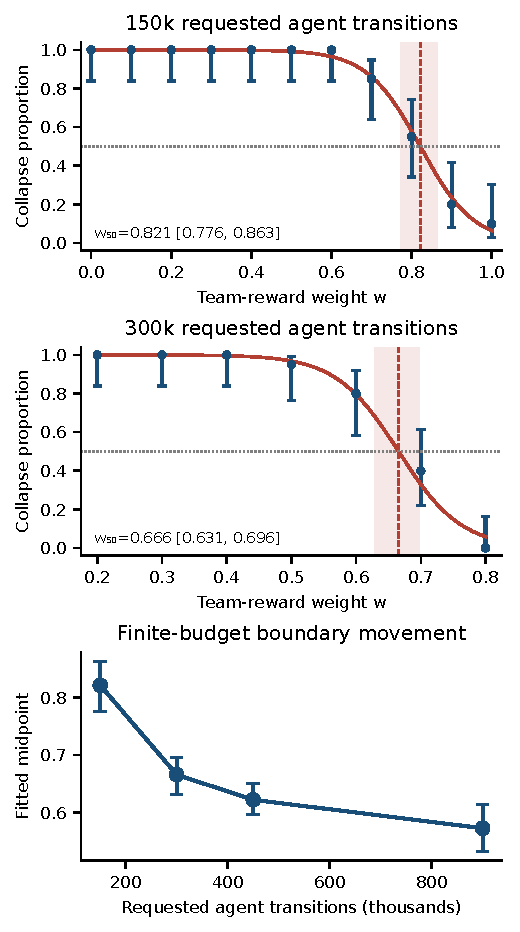
\includegraphics[width=.62\textwidth]{generated/boundary_observed.pdf}
\caption{Finite-budget supply PPO crossings. Top and middle: observed collapse proportions with 95\% Wilson intervals, Firth curves drawn only over sampled grids, midpoint lines and seed-block 95\% CI bands. Bottom: independently fitted horizons; budgets count requested agent transitions.}
\label{fig:boundary}
\Description{Observed collapse proportions and fitted curves at 150k and 300k, followed by the four estimated finite-budget midpoints and intervals.}
\end{figure}

\section{Training-Budget Dependence}
\label{sec:horizon}
\paragraph{The boundary is finite-horizon.}
The boundary slides left across four linear-reward budgets: the recomputed
midpoints are 0.821, 0.666, 0.622 and 0.572 at 150/300/450/900k requested agent
transitions (Figure~\ref{fig:boundary}).
These are separate finite-budget estimates; neither a nonzero asymptote nor
within-policy recovery follows from this cross-sectional comparison.


\paragraph{Independent longitudinal confirmation.}
After 120 pilot trajectories, we froze five common cells $w\in\{.2,.4,.6,.85,1\}$ and ten disjoint confirmation seeds per cell for linear, curvature-only and $\lambda=7$ rewards: 150 trajectories to 3.6M, evaluated every 150k. The loss-multiplier-minus-curvature crossing difference remains positive at all four primary budgets: $+.281$ $[.174,.363]$, $+.284$ $[.182,.393]$, $+.326$ $[.222,.433]$, and $+.146$ $[.072,.229]$ at 300k, 900k, 1.8M, and 3.6M (Figure~\ref{fig:confirmation}a). These pointwise seed-block intervals support persistence over the tested budgets, not an infinite-horizon limit. None of the three conditions meets the declared practical-stability criterion: the entire interval for its 3.6M-minus-1.8M change must lie within $[-.02,.02]$.
At 1.8M, the absolute crossings are $.589$ $[.500,.698]$ (linear), $.399$ $[.291,.503]$ (curvature), and $.725$ $[.725,.725]$ (loss multiplier); at 3.6M they are $.590$ $[.482,.700]$, $.524$ $[.420,.630]$, and $.670$ $[.604,.725]$. The crossing has not demonstrably stopped moving. The zero-width 1.8M multiplier interval reflects identical seed-label patterns on a coarse grid, not exact localization.

\paragraph{Recovery and evaluation sensitivity.}
Checkpoints track the same policies, permitting recovery and relapse analysis conditional on the 300k label. Across the fixed grid, 6/27 linear, 4/23 curvature-only and 7/35 lambda-7 trajectories collapsed at 300k are noncollapsed at 3.6M; among initially noncollapsed trajectories, 3/23, 2/27 and 0/15 respectively relapse. These descriptive totals are stratified by mixture cell in Appendix~\ref{app:confirmation}, alongside three-checkpoint recovery and subsequent relapse. Increasing evaluation from ten to fifty episodes at 900k, 1.8M and 3.6M changes only one of 450 labels and leaves the 3.6M contrast unchanged. Coarsening has a cost: identical seed-label patterns give zero-width bootstrap intervals at several $\lambda=7$ checkpoints, including 900k and 1.8M. Their observed crossing bracket is still $[.6,.85]$; bootstrap degeneracy does not imply exact localization. Appendix~\ref{app:confirmation} gives full checkpoint curves, cell support and sensitivity tables.

\begin{figure}[t]
\centering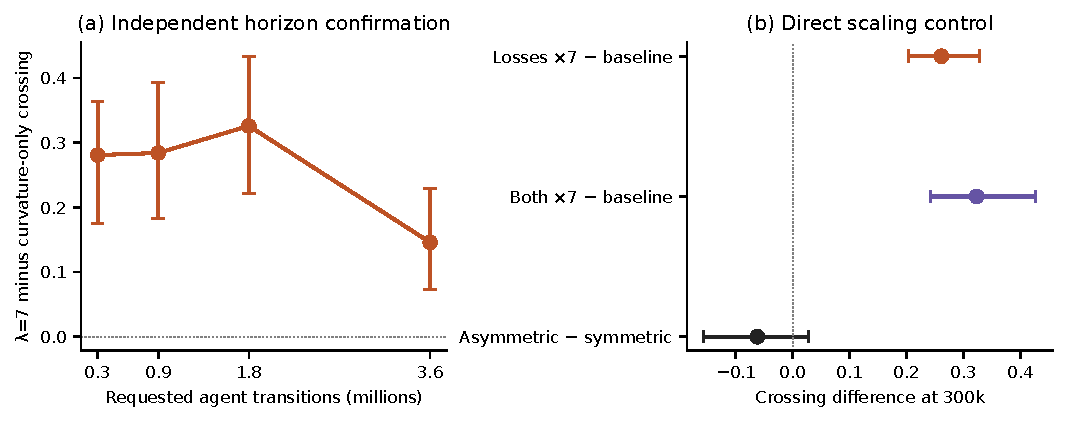
\includegraphics[width=\textwidth]{generated/confirmation/confirmed_effects.pdf}
\caption{Independent confirmation with ten paired training seeds and 2,000 seed-block bootstrap draws. (a) Loss-multiplier-minus-curvature crossing differences at four declared budgets, using five common mixture cells and reference zero. (b) Three-arm control at 300k on eight cells, with a shared empirical-mean reference: both asymmetric and symmetric multipliers shift the crossing relative to curvature-only, while their direct difference includes zero. Intervals are pointwise; the two panels use different fixed references and are not pooled.}
\label{fig:confirmation}
\Description{The horizon contrast remains positive through 3.6 million transitions. Both control arms differ positively from baseline, while the asymmetric-minus-symmetric interval crosses zero.}
\end{figure}

\section{Reward-Transform Comparisons}
\label{sec:transforms}
\paragraph{The selected loss-multiplier shift opposes curvature.}
Two baselines anchor the comparison, all with identical environment, learner, label, and 300k
horizon. The linear null ($\alpha{=}\beta{=}1,\lambda{=}1$) was measured twice as a reproducibility
check (\Headline{} in the main structural sweep and \RepeatedNull{} in the
independent decomposition run, overlap does not establish equivalence; the decomposition uses its own linear run); the second is the curvature baseline
($\alpha{=}\beta{=}0.88,\lambda{=}1$), fixed at the conventional prospect-theory curvature
estimate~\citep{tversky1992}, not tuned; the sweep then varies only $\lambda\in\{1,\dots,7\}$. The
selected high-minus-low endpoint is positive, with high-lambda estimates near $0.85$ within the sampled grid ( Figure~\ref{fig:decomposition}, Table~\ref{tab:decomposition}). Curvature alone acts in the
\emph{opposite} direction, lowering $\wcrit$ to $0.585$ ($-0.100$ $[-0.145,-0.057]$ vs.\ linear), which
is why we decompose: as a single ``prospect-theoretic'' treatment the two effects partially cancel,
since here curvature lowers the measured crossing while the loss multiplier raises it.

\paragraph{Two effect sizes answer two questions.}
The effect size depends on the baseline (Table~\ref{tab:decomposition}). The \emph{full-transform shift}
against the linear baseline is the total change a designer sees adopting the full transform; the
\emph{loss-multiplier shift} against the curvature baseline is the cleaner estimate of the
$\lambda$ effect,
since curvature is present in every sweep condition, and the two differ by the curvature offset
($-0.100$). Throughout, the loss-multiplier effect denotes this increment; it does not by itself identify gain--loss asymmetry.

\paragraph{Reference and scale sensitivity.}
The loss multiplier changes both sign weighting and reward scale. A fixed pilot-RMS control leaves a recomputed endpoint difference of $+.145$ $[.108,.186]$, but fixed calibration does not ensure achieved on-policy RMS or advantage matching. The common reward-unit coordinate $q=wc_g/[(1-w)c_\ell+wc_g]$, where $c_\ell,c_g$ are applied unit multipliers, also retains a local-unit difference of $+.053$ $[.009,.100]$ at lambda 1. We therefore completed a direct three-arm comparison on eight mixture cells with ten seeds each, holding $z_0=-2.6281398333$ fixed from 60,000 independent calibration samples. With $u=x-z_0$ and $\phi(u)=\mathrm{sign}(u)|u|^{.88}$, the arms are $B=\phi(u)$, $A=v_7(u)$ and $S=7\phi(u)$. Their crossings are .560, .821 and .883. Relative to B, A shifts the crossing by $+.261$ $[.203,.329]$ and S by $+.323$ $[.241,.427]$; the direct A--S difference is $-.062$ $[-.157,.028]$ (Figure~\ref{fig:confirmation}b). This does not establish an asymmetry-specific effect or equivalence between arms.

Both gain and loss branches are active: near-crossing loss fractions are 34.0\%, 31.1\% and 20.4\% for B, A and S. Nevertheless, pooled transformed-reward RMS values are 8.80, 30.36 and 57.67, and raw advantage SDs are 35.05, 135.95 and 300.40. Normalized optimizer advantages have almost identical SD (.99765), but every control minibatch triggers global gradient clipping, with critic gradients dominating. This leaves an optimizer-scaling pathway despite advantage normalization; it is not a causal diagnosis. Appendix~\ref{app:direct_control} gives observed cells, intervals and training diagnostics.

\begin{figure}[t]
\centering
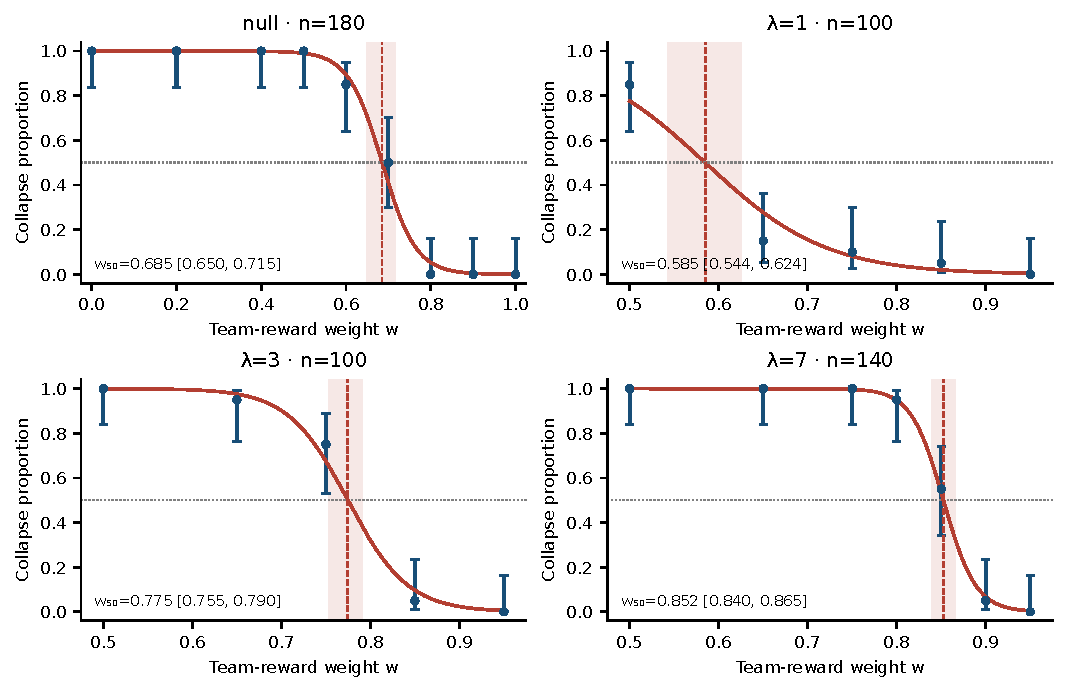
\includegraphics[width=.92\textwidth]{generated/decomposition_observed.pdf}
\caption{Supply PPO null and selected transform conditions at 300k. Points show collapse counts divided by cell totals with 95\% Wilson intervals; curves are Firth fits over observed grids. Vertical bands are midpoint seed-block intervals. The lambda-7 panel includes the completed $w=.8,.9$ refinements; Appendix~\ref{app:estimation} reports the full sweep counts.}
\label{fig:decomposition}
\Description{Four panels compare observed collapse proportions and fitted midpoints for null, lambda one, lambda three and lambda seven.}
\end{figure}

\begin{table*}[t]
\caption{Supply-PPO reward-transform decomposition at 300k requested agent transitions and descriptive equivalent linear-training budgets. Differences use paired seed-block draws. Equivalent budgets invert the four-point cross-sectional fit $w_{50}=1.4824-0.13748\log(T/1000)$ and propagate the same 2,000 bootstrap replicates; they are descriptive, not causal. $\dagger$ denotes extrapolation below the observed 150k--900k horizon range.}
\label{tab:decomposition}
\centering\small
{\setlength{\tabcolsep}{4pt}
\begin{tabular}{@{}lllll@{}}
\toprule
Condition & Crossing and 95\% CI & Versus null & Versus curvature & Equivalent budget, k \\
\midrule
Linear null & $0.685$ $[0.650,0.715]$ & -- & -- & $330$ $[275,406]$ \\
Curvature ($\lambda=1$) & $0.585$ $[0.544,0.624]$ & $-0.100$ $[-0.145,-0.057]$ & -- & $685$ $[535,942]$ \\
$\lambda=3$ & $0.775$ $[0.755,0.790]$ & $+0.090$ $[+0.065,+0.115]$ & $+0.190$ $[+0.150,+0.229]$ & $172$ $[140,211]$ \\
$\lambda=7$ & $0.852$ $[0.840,0.865]$ & $+0.167$ $[+0.134,+0.203]$ & $+0.268$ $[+0.230,+0.306]$ & $98$ $[67,128]$$^{\dagger}$ \\
\bottomrule
\end{tabular}
}
\end{table*}


\paragraph{Equivalent linear-training budget.}
As a descriptive effect-size translation, we fit the four cross-sectional linear estimates to
$w_{50}=1.4824-0.13748\log(T/1000)$ and invert that curve for each transform crossing. Curvature-only
at 300k maps to a linear budget of 685k $[535,942]$, whereas $\lambda=7$ maps to 98k $[67,128]$;
the repeated linear null maps to 330k $[275,406]$. Thus the observed $\lambda=7$ crossing resembles
roughly one third of the nominal linear-training budget under this local empirical mapping. The
$\lambda=7$ value extrapolates below the observed 150k--900k horizon range, and none of these mappings
identifies a causal equivalence.

The curvature result is scoped to supply-chain PPO. A loss-multiplier effect is a property of the transformed training signal; the completed direct control does not identify a sign-dependent effect beyond scalar scaling. Neither an endpoint difference nor the hypothetical SNR account supplies that identification on its own.

% =======================================================================
\paragraph{Cost and normalization.}
A five-cell, 20-seed boundary requires 100 trained policies. Retrospective fixed-grid thinning saves 20--40\% of runs in the tested 20-seed comparisons, but can change the midpoint by .074; it does not validate an adaptive design or guarantee accuracy in a new domain. Confirmation consumed 530.57 CPU-hours for the horizon cohort and 61.38 for direct controls, including evaluation and checkpointing. Appendix~\ref{app:compute} reports elapsed time, pilot costs and memory. Fix local/team units, sum-versus-average aggregation and reference transformation before comparison; the common $q$ coordinate does not remove optimizer-scale sensitivity.

% =======================================================================
\section{Discussion}
\label{sec:discussion}

Separating curvature from the loss multiplier gives opposing crossing shifts on supply-chain PPO, but does not separate asymmetry from optimizer-scale effects. The independent long-horizon comparison retains a positive multiplier contrast through 3.6M; the empirical-mean direct control also finds a positive shift under symmetric scaling. Together these results support the measurement instrument and the budget-conditional transform comparison, while leaving an asymmetry-specific mechanism unestablished.

The crossing is a diagnostic of the specified training and evaluation procedure.
A deployment requirement such as at most 5\% collapse would need its own
probability target and uncertainty assessment; the 50\% midpoint supplies no
such guarantee. The collapse definition and its observed behavioral components are reported in
Appendix~\ref{app:configuration}.

\paragraph{Scope and Future Work.}
Three limits point to next steps. The quantitative core is single-substrate, so magnitudes belong to
one simulator and must be re-estimated elsewhere. The direct control does not isolate asymmetry from
scale, and critic-dominated global clipping supplies a concrete but untested causal pathway. A targeted
optimizer intervention is therefore more informative than another descriptive transform sweep.
Which implementation choices make collapse persistent is not identified by these data; resolving that
question requires common-code ablations rather than comparison with a separately rebuilt pipeline. Our
crossing therefore conditions explicitly on the policy architecture, joint clipping, rollout rounding,
observation wrapper, and simulator stream recorded in Appendix~\ref{app:configuration}.
Localizing $\wcrit$ from dynamics also resisted two probes, so a predictive observable remains an open
problem. The common reward-unit coordinate retains measured differences; fixed units and aggregation
conventions remain part of the protocol. Retrospective grid thinning saves runs but can move
the midpoint appreciably (up to .074 for the tested 20-seed primary thinning rule);
this is not evidence of universally cheap boundary estimation.

% =======================================================================
\section{Conclusion}
\label{sec:conclusion}

Reward centralization is usually treated as a direction: more team signal helps. We show that it also
has a measurable finite-budget location, $\wcrit$, and that the estimated crossing changes with reward
transforms and training budget. Independent confirmation retains a multiplier-minus-curvature shift
through 3.6M transitions, but a symmetric-scaling control moves the crossing at least as far as the
loss-only multiplier. The evidence therefore supports a comparative measurement protocol and a
reward-scale sensitivity result, not a gain--loss-asymmetry mechanism. The numerical threshold remains
conditional on the environment, learner, optimizer, budget, reward units, and behavioral label.

% =======================================================================
\section*{Ethical Statement}

This work is entirely simulated, with no human subjects or personal data. Reported thresholds are
substrate-specific and must be re-measured before use.

% =======================================================================
